\title{Lecture 11\\A Basic Programming Language for Knowledge Base Processing}

\begin{frame}
	\titlepage
\end{frame}

\begin{frame}{\\Lecture outline}
	\topline
	\RaggedRight
	Basic principles of knowledge processing. One-, two- and three-element constructions. Arbitrary constructions; pattern-based search and generation. Fundamentals of SCP. scp-programs, scp-processes and scp-operators. scp-operands and their classification; scp-variables and scp-constants. Classification of scp-operators. Conditional and unconditional branching, loops. Subroutines. Agent scp-programs.

\end{frame}

\begin{frame}{\\SCP language}
	\topline
	\RaggedRight
	\vspace{1.5em}
	\begin{SCn}
		\scnheader{SCP language}
		\scnidtftext{commonly used sc-identifier}{scp-program}
	\end{SCn}
		\scntext{explanation}{\small The proposed basic language for describing programs that process texts in
			\textit{SC-code} is the \textit{SCP language}.

			\textit{SCP language} is a graph-based procedural programming language
designed for efficient processing of \textit{sc-texts}. \textit{SCP language} is a parallel asynchronous programming language.

The data representation language for texts in the \textit{SCP language}
			(\textit{scp-programs}) is \textit{SC-code} and, accordingly, any of its external representations.

			\textit{SCP language} is considered an assembly language for a semantic computer.}
		\end{frame}

\begin{frame}{\\Storing and processing SC-code}%
\topline
\RaggedRight
\vspace{1.5em}
\begin{SCn}
	\scnheader{SC-code}
	\scnidtf{Semantic Computer Code}
\end{SCn}

\scntext{note}{\textit{SC-code} has fixed syntax and denotational semantics, but variable operational semantics. It can therefore serve as a basis for a family of knowledge representation languages of different kinds.

\textit{SC-code} was originally designed as a language for encoding information in the memory of \textit{semantic associative computers}. It therefore incorporates universality (the ability to represent any kind of knowledge), uniformity of representation, and minimization of the \textit{SC-code alphabet}, which facilitates the development of hardware for storing and processing texts in \textit{SC-code}.}
\end{frame}

\begin{frame}{\\Abstract scp-machine}%
		\topline
		\RaggedRight
		\begin{SCn}
			\scnheader{Abstract scp-machine}
			\scniselement{scp-machine}\scnrelto{generalized model}{scp-interpreter
			}
		\end{SCn}
			\scntext{note}{The \textit{Abstract scp-machine} is an interpreter for \textit{scp-programs} that must be part of the \textit{ostis-platform} (although platform variants without such an interpreter may exist, they cannot exploit the proposed basic execution model).}
	\end{frame}

\begin{frame}{Types of sc-structures\\ from the processing perspective}
	\topline
	\RaggedRight
	\begin{SCn}
	\scnheader{sc-structure}
	\begin{scnrelfromset}{partition}
	\scnitem{sc-construction of a non-standard form}
	\scnitem{sc-construction of a standard form}
	\begin{scnindent}
		\begin{scnrelfromset}{partition}
			\scnitem{one-element sc-construction}
			\scnitem{three-element sc-construction}
			\scnitem{five-element sc-construction}
		\end{scnrelfromset}
	\end{scnindent}
	\end{scnrelfromset}
	\end{SCn}
\end{frame}

\begin{frame}{\\sc-construction of a non-standard form}
	\topline
	\RaggedRight
	\begin{SCn}
		\scnheader{sc-construction of a non-standard form}
		\scntext{explanation}{Each \textit{sc-construction of a non-standard form} consists of an arbitrary number of \textit{sc-elements} of arbitrary types.}
		\scnrelfrom{example}{
			\begin{center}
				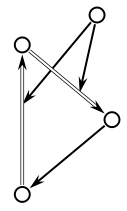
\includegraphics[width=18mm]{figures/sd_scp/pic_ps1.png}
		\end{center}}
	\end{SCn}
\end{frame}

\begin{frame}{\\sc-construction of a standard form}
	\topline
	\RaggedRight
	\begin{SCn}
		\scnheader{sc-construction of a standard form}
		\scntext{explanation}{In turn, each element of a \textit{\mbox{sc-construction} of a standard form} has a strictly fixed relative position within that \mbox{sc-construction} (first element, second element, etc.). Depending on that position, additional restrictions are imposed on the type of the corresponding \textit{sc-element}.}
	\end{SCn}
\end{frame}

\begin{frame}{\\One-element sc-construction}
	\topline
	\RaggedRight
	\begin{SCn}
		\scnheader{one-element sc-construction}
		\scntext{explanation}{Each \textit{one-element sc-construction} consists of one \newline \textit{sc-element} of an arbitrary type.}
		\scnrelfrom{example}{
			\begin{center}
				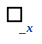
\includegraphics[width=17mm]{figures/sd_scp/pic_ps2.png}
		\end{center}}
	\end{SCn}
\end{frame}

\begin{frame}{\\Three-element sc-construction}
	\topline
	\RaggedRight
	\begin{SCn}
		\scnheader{three-element sc-construction}
		\scntext{explanation}{Each \textit{three-element sc-construction} consists of three \newline \textit{sc-elements}. The second element is always an \textit{sc-connector}; the other elements may be of arbitrary types.}
		\scnrelfrom{example}{
			\begin{center}
				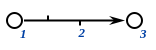
\includegraphics[width=35mm]{figures/sd_scp/pic_ps3.png}
		\end{center}}
	\end{SCn}
\end{frame}

\begin{frame}{\\Five-element sc-construction}
	\topline
	\RaggedRight
	\begin{SCn}
		\scnheader{five-element sc-construction}
		\scntext{explanation}{Each \textit{five-element sc-construction} consists of five \newline \textit{sc-elements}. The second and fourth elements must be \textit{sc-connectors}; the other elements may be of arbitrary types.}
		\scnrelfrom{example}{
			\begin{center}
				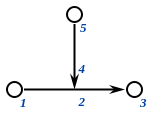
\includegraphics[width=35mm]{figures/sd_scp/pic_ps4.png}
		\end{center}}
	\end{SCn}
\end{frame}


\begin{frame}{\\scp-program}%
	\topline
	\RaggedRight
	\begin{SCn}
		\scnheader{scp-program}
		\scnsubset{program in sc-memory}
		\scnsuperset{agent scp-program}
		\end{SCn}
\scntext{explanation}{Each \textbf{\textit{scp-program}} is a \textit{generalized structure} that describes one way of decomposing actions of a class executed in sc-memory. The sign of the \textit{sc-variable} corresponding to the particular action being decomposed is, within the \textbf{\textit{scp-program}}, the \textit{key sc-element\scnrolesign}.

Essentially, each \textbf{\textit{scp-program}} describes a sequence of elementary operations on a semantic network required to perform a more complex action of a given class.}
\end{frame}

\begin{frame}%
	\scntext{example description}{
	\begin{center}
	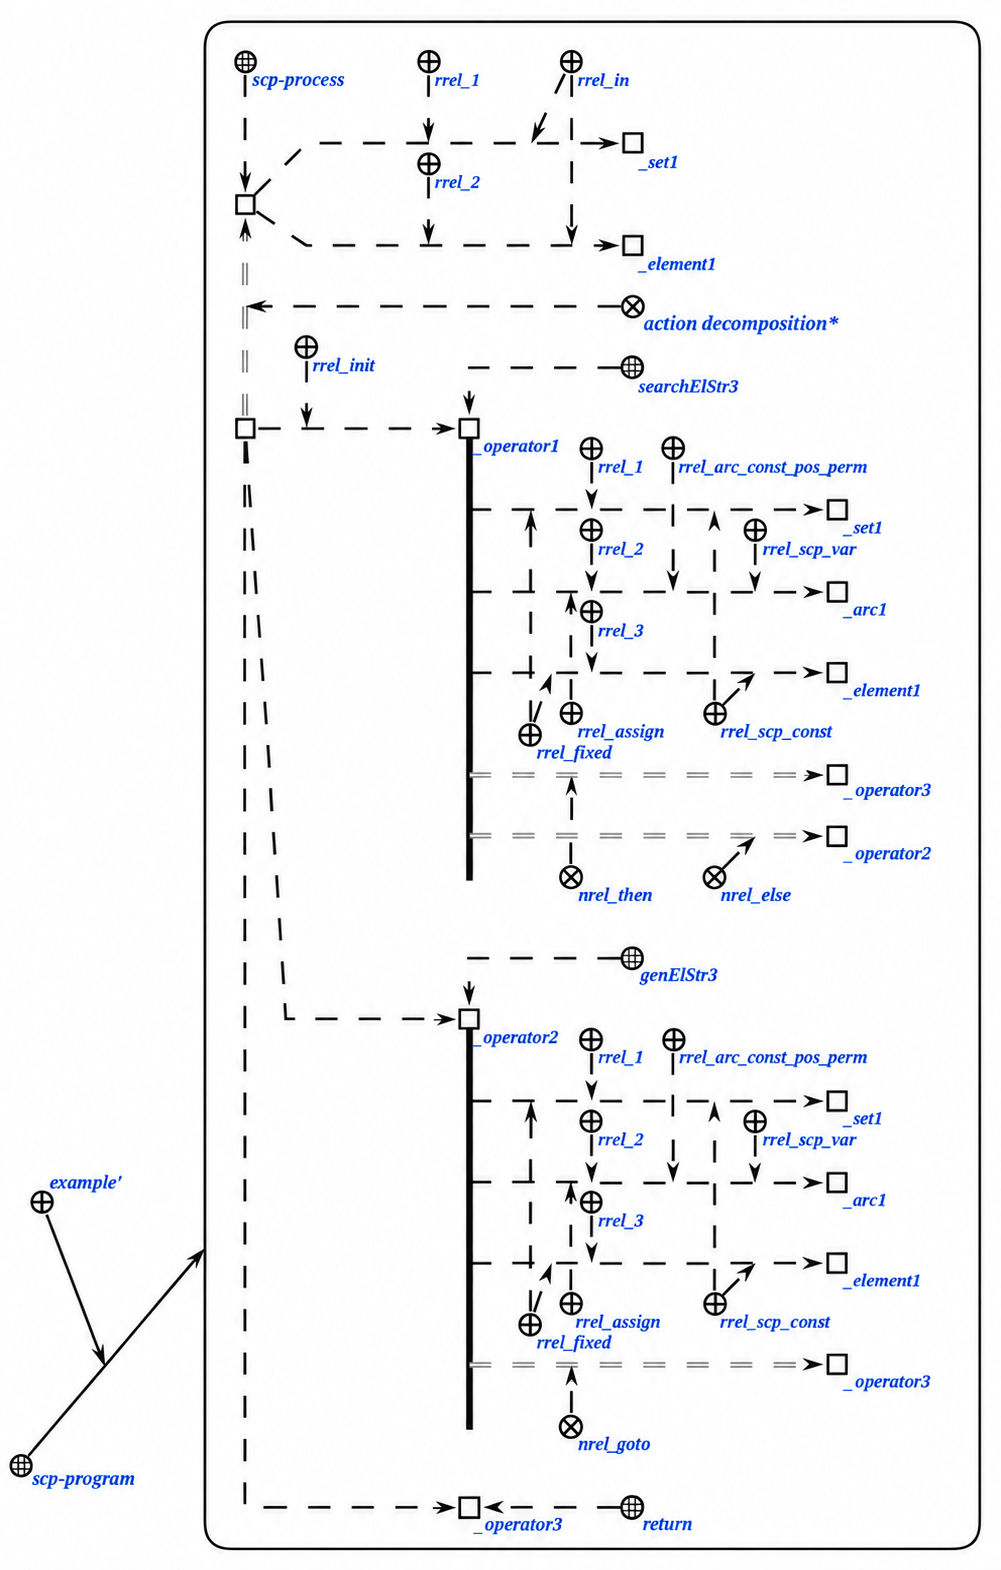
\includegraphics[width=127.56bp,height=200.08bp,keepaspectratio]{figures/sd_scp/program_example_en.png}
	\end{center}}
\end{frame}

\begin{frame}%
			\scntext{explanation}{The example shows an \textit{scp-program} consisting of three \textit{scp-operators}. It checks whether a given set (the first parameter) contains a given element (the second parameter), and adds it to the set if it does not.}
\end{frame}

\begin{frame}{\\scp-process}%
	\topline
	\RaggedRight
		\scnheader{scp-process}
		\scntext{explanation}{\RaggedRight A \textbf{\textit{scp-process}} is understood as an \textit{action in sc-memory} that unambiguously describes a particular execution of an \textit{scp-program} for given input data. While an \textit{scp-program} describes a general algorithm for solving a task, an \textit{scp-process} denotes a specific action implementing that algorithm for given input parameters.

Essentially, each \textbf{\textit{scp-process}} is a unique copy of an \textit{scp-program}. Each \textit{sc-variable}, except for \textit{scp-variables\scnrolesign}, is replaced by a generated \textit{sc-constant}. An action's membership in the set of \textit{scp-processes} guarantees that its decomposition contains only signs of elementary actions (\textit{scp-operators}) that the implementation of the \textit{Abstract scp-machine} can interpret.}
		\vspace{-2em}
		\end{frame}

\begin{frame}%
		\scntext{execution example}{
			\begin{center}
			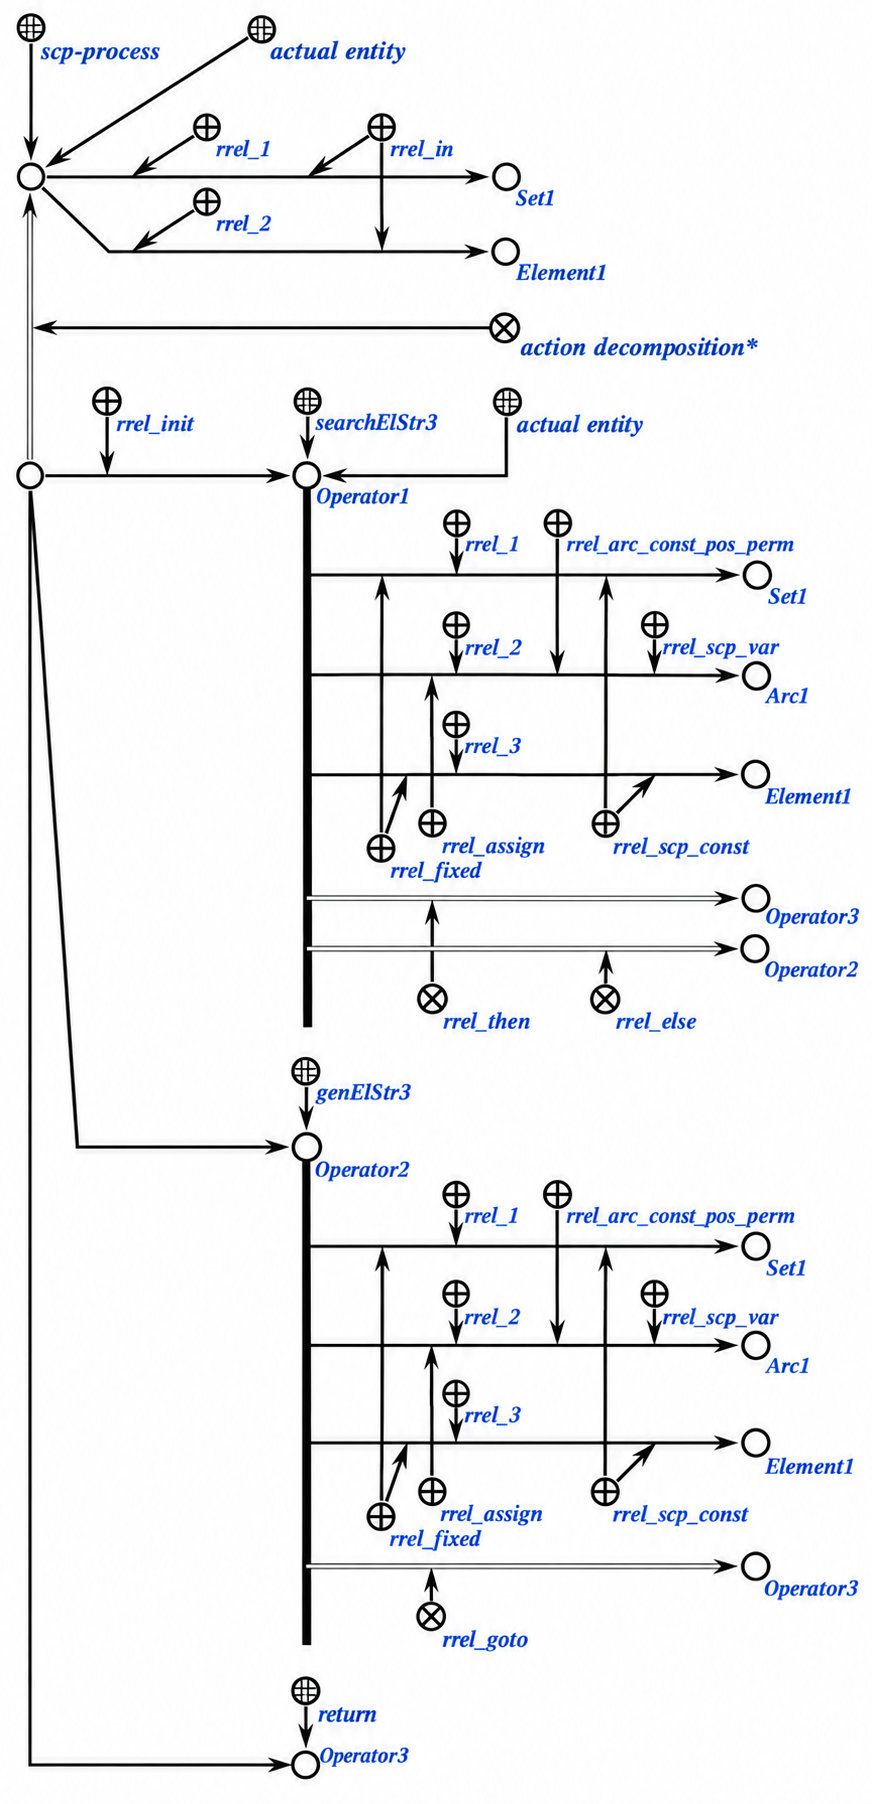
\includegraphics[width=96.38bp,height=199.55bp,keepaspectratio]{figures/sd_scp/process_example_en.png}
		\end{center}}
\end{frame}

\begin{frame}%
			\scntext{explanation}{The \textit{scp-program} is called. The corresponding \textit{scp-process} is generated. The initial scp-process operator, \textit{Operator1}, is initiated.}
\end{frame}

\begin{frame}{\\Structure of an scp-process}%
	\topline
	\RaggedRight
	\begin{textitemize}
		\item \textit{scp-operators}
		\item connections specifying the execution order \textit{scp-operators}
		\item arguments \textit{scp-process} (\textit{scp-program})
	\end{textitemize}
	\vspace{-2em}
\end{frame}

\begin{frame}{\\scp-operator}%
	\topline
	\RaggedRight

	\begin{SCn}
		\scnheader{scp-operator}
		\scntext{explanation}{Each \textbf{\textit{scp-operator}} is an elementary \textit{action in sc-memory}. The arguments of an \textit{scp-operator} are called operands. Their order is specified by the corresponding role relations (\textit{1\scnrolesign}, \textit{2\scnrolesign}, \textit{3\scnrolesign} and so on). An operand marked by the role relation \textit{1\scnrolesign} is called the first operand; one marked by the role relation \textit{2\scnrolesign} is the second operand, and so on. The type and meaning of each operand are further specified by subclasses of the \textit{scp-operand\scnrolesign} relation. In general, an operand can be any \textit{sc-element} including the sign of an \textit{scp-program}, including the program containing this operator.}
	\end{SCn}
\end{frame}


\begin{frame}{\\scp-operator}%
	\topline
	\RaggedRight

	\begin{SCn}
		\scnheader{scp-operator}
		\scntext{note}{Each \textbf{\textit{scp-operator}} must have one or more operands and an indication of the \textbf{\textit{scp-operator}} (or several operators) to execute next. The exception is the \textit{scp-operator for program termination} which has no operands and after which no \textit{scp-operators} can be executed within that program.}
\end{SCn}
\end{frame}

\begin{frame}{\\scp-operator}%
	\topline
	\RaggedRight
	\begin{SCn}
		\scnheader{scp-operator}
		\scnsubset{action in sc-memory}
				\scnrelto{family of subsets}{atomic type of scp-operator}
				\begin{scnrelfromset}{partition}
					\scnitem{scp-operator for construction generation}
					\scnitem{scp-operator for associative construction search}
					\scnitem{scp-operator for construction deletion}
					\scnitem{scp-operator for condition checking}
					\scnitem{scp-operator for operand value management}
					\scnitem{scp-operator for scp-process management}
					\scnitem{scp-operator for event management}
					\scnitem{scp-operator for file content processing}
					\scnitem{scp-operator for lock management}
				\end{scnrelfromset}
	\end{SCn}
	\vspace{-2 em}
\end{frame}

\begin{frame}{\\scp-operator for construction generation}%
	\topline
	\RaggedRight
	\begin{SCn}

		\scnheader{scp-operator for construction generation}
		\begin{scnrelfromset}{partition}
			\scnitem{scp-operator for generating a construction from an arbitrary pattern}
			\scnitem{scp-operator for five-element construction generation}
			\scnitem{scp-operator for three-element construction generation}
			\scnitem{scp-operator for one-element construction generation}
		\end{scnrelfromset}

	\end{SCn}
	\vspace{-2 em}
\end{frame}

\begin{frame}{scp-operator for associative construction search}%
	\topline
	\RaggedRight
	\begin{SCn}

	\scnheader{scp-operator for associative construction search}
	\begin{scnrelfromset}{partition}
		\scnitem{scp-operator for searching for a construction using an arbitrary pattern}
		\scnitem{scp-operator for five-element construction search with set formation}
		\scnitem{scp-operator for three-element construction search with set formation}
		\scnitem{scp-operator for five-element construction search}
		\scnitem{scp-operator for three-element construction search}
	\end{scnrelfromset}

	\end{SCn}
	\vspace{-2 em}
\end{frame}

\begin{frame}{\\Atomic type of scp-operator}%
	\topline
	\RaggedRight
	\begin{SCn}
		\scnheader{atomic type of scp-operator}
		\scntext{explanation}{Each \textbf{\textit{atomic type of scp-operator}} is a class of \textit{scp-operators} that is not partitioned into more specific classes and is therefore interpreted by the implementation of the \textit{Abstract scp-machine}. }
		\end{SCn}
\end{frame}

\begin{frame}{\\Decomposition of an scp-process}%
	\topline
	\RaggedRight

	\begin{center}
		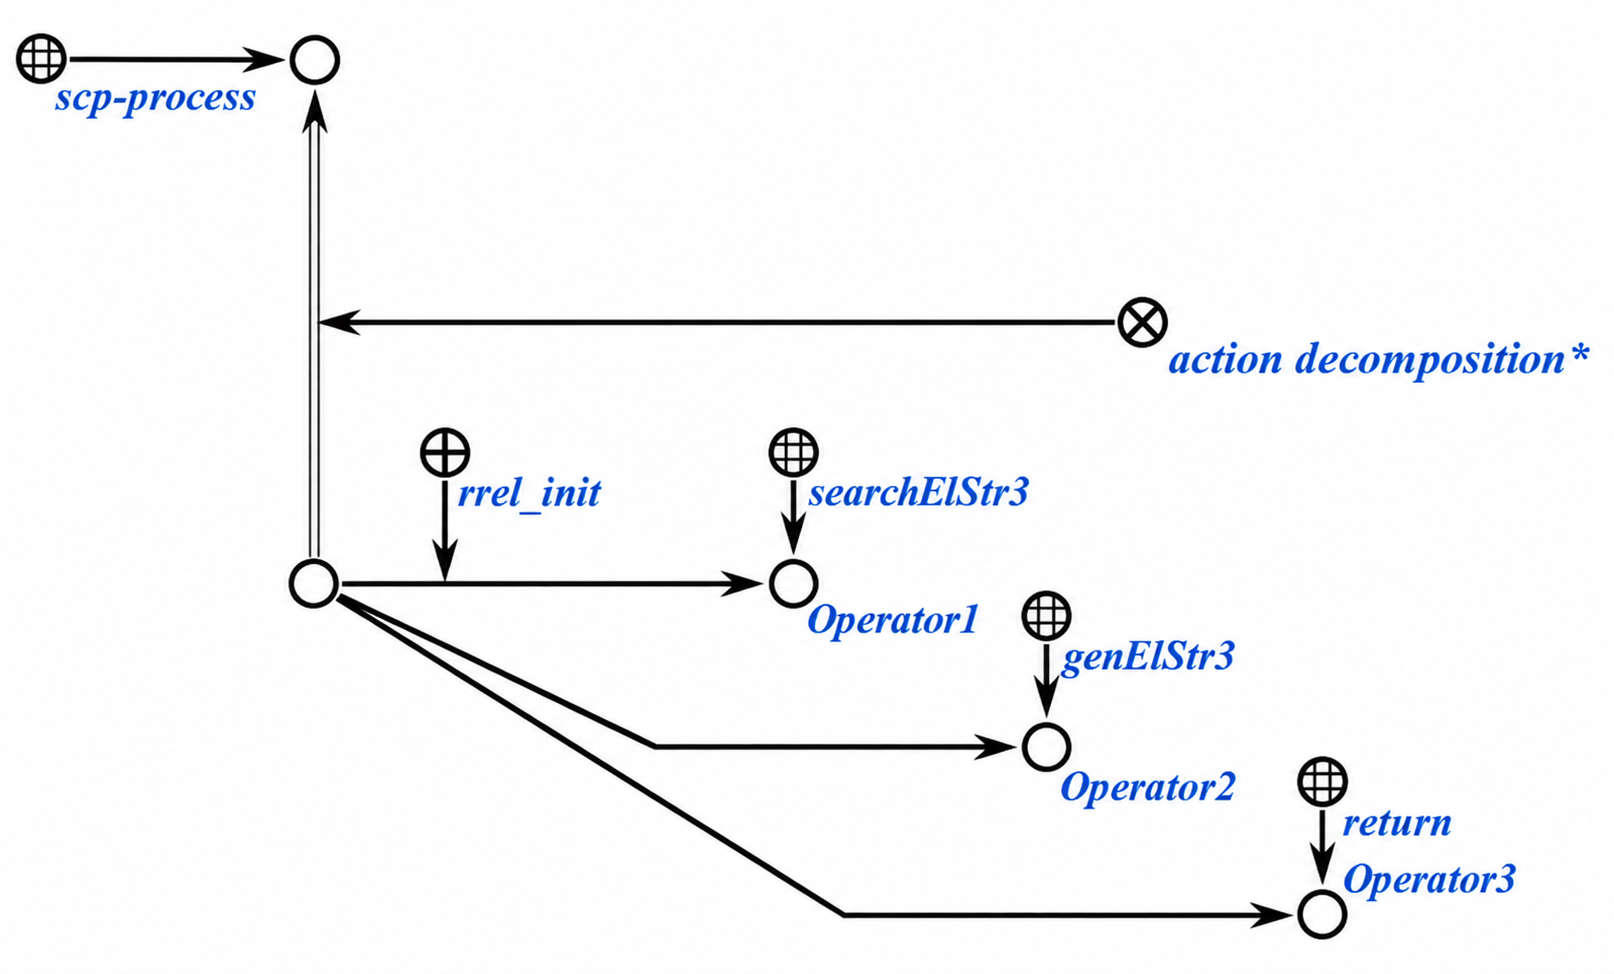
\includegraphics[width=283.48bp,height=171.11bp,keepaspectratio]{figures/sd_scp/process_decomp_en.png}
	\end{center}

	\vspace{-2em}
\end{frame}

\begin{frame}{\\Initial scp-operator}%
	\topline
	\RaggedRight
	\begin{SCn}
		\scnheader{initial operator\scnrolesign}
		\scnsubset{1\scnrolesign}
		\scntext{explanation}{The role relation \textbf{\textit{initial operator\scnrolesign}} identifies, within the decomposition of the \textit{scp-process} corresponding to an \textit{\mbox{scp-program}}, the \textit{scp-operators} that must be executed first, i.e., those that begin execution of the \textit{scp-process}.}
		\end{SCn}
	\end{frame}

\begin{frame}{\\scp-operand}%
	\topline
	\RaggedRight
		Each \textit{scp-operator} is a set of \textit{scp-operands}. Role relations specify the role of each scp-operand within the corresponding \textit{scp-operator}.

		\begin{SCn}
		\scnheader{scp-operand\scnrolesign}
		\scntext{explanation}{The role relation \textit{scp-operand\scnrolesign} is a non-basic concept and specifies that arguments belong to an \textit{scp-operator}. In addition to specifying a class of \textit{scp-operands\scnrolesign}, the order of the arguments of an \textit{scp-operator} is further specified by \textit{the role relations 1\scnrolesign}, \textit{2\scnrolesign} and so on.}
		\end{SCn}

	\vspace{-2.3em}
\end{frame}

\begin{frame}{\\scp-operand}%
	\topline
	\RaggedRight
	\footnotesize
	\begin{SCn}
		\scnheader{scp-operand\scnrolesign}
		\scniselement{non-basic concept}
		\scniselement{role relation}
		\begin{scnrelfromset}{partition}
			\scnitem{scp-variable\scnrolesign}
			\scnitem{scp-constant\scnrolesign}
			\end{scnrelfromset}
		\begin{scnrelfromset}{partition}
			\scnitem{scp-operand with an assigned value\scnrolesign}
			\begin{scnindent}
				\scntext{system identifier}{rrel\_fixed}
			\end{scnindent}
			\scnitem{scp-operand with an unassigned value\scnrolesign}
				\begin{scnindent}
				\scntext{system identifier}{rrel\_assign}
			\end{scnindent}
		\end{scnrelfromset}
	\begin{scnrelfromset}{partition}
		\scnitem{constant sc-element\scnrolesign}
		\scnitem{variable sc-element\scnrolesign}
	\end{scnrelfromset}
	\end{SCn}
\vspace{-2.3em}
\end{frame}

\begin{frame}{\\scp-variable}%
	\topline
	\RaggedRight
	\begin{SCn}
		\scnheader{scp-variable\scnrolesign}
		\scntext{explanation}{Within an \textit{scp-program}, \textit{scp-variables\scnrolesign} are not processed explicitly during interpretation; their values are processed instead. Each variable of an \textit{scp-program} can have one value at a time, i.e., it is a situational \textit{singleton} whose element is the current value of the \textit{scp-variable\scnrolesign}. The value of each \textit{scp-variable\scnrolesign} may change during interpretation of the \textit{scp-program}. When processing an \textit{scp-operator}, the interpreter works directly with the values of \textit{\mbox{scp-variables\scnrolesign}} rather than the \textit{scp-variables\scnrolesign} themselves (which are also nodes in the same semantic network).}
	\end{SCn}
\end{frame}

\begin{frame}{\\scp-constant}%
	\topline
	\RaggedRight
	\small

	\begin{SCn}
		\scnheader{scp-constant\scnrolesign}
		\scntext{explanation}{Within an \textit{scp-program}, \textit{scp-constants\scnrolesign} participate explicitly in \textit{\mbox{scp-operators}} as elements (in the set-theoretic sense) and are processed directly during interpretation of the \textit{scp-program}. Constants within an \textit{scp-program} can be \textit{sc-elements} of any type, both \textit{\mbox{sc-constants}} and \textit{\mbox{sc-variables}}. A constant within an \textit{scp-program} remains unchanged throughout interpretation. A constant of an \textit{\mbox{scp-program}} can be considered a variable whose value always equals the variable itself and cannot be changed. Henceforth, we treat an \textit{scp-constant\scnrolesign} and its value as the same entity. Each \textit{in-parameter\scnrolesign} during interpretation of each particular copy of an \textit{scp-program} becomes an \textit{scp-constant\scnrolesign} within all its operators, although in the original program body it is an \textit{scp-variable\scnrolesign}.}
	\end{SCn}
\end{frame}

\begin{frame}{\\Example of using scp-variables}%
	\topline
	\RaggedRight

	\begin{center}
		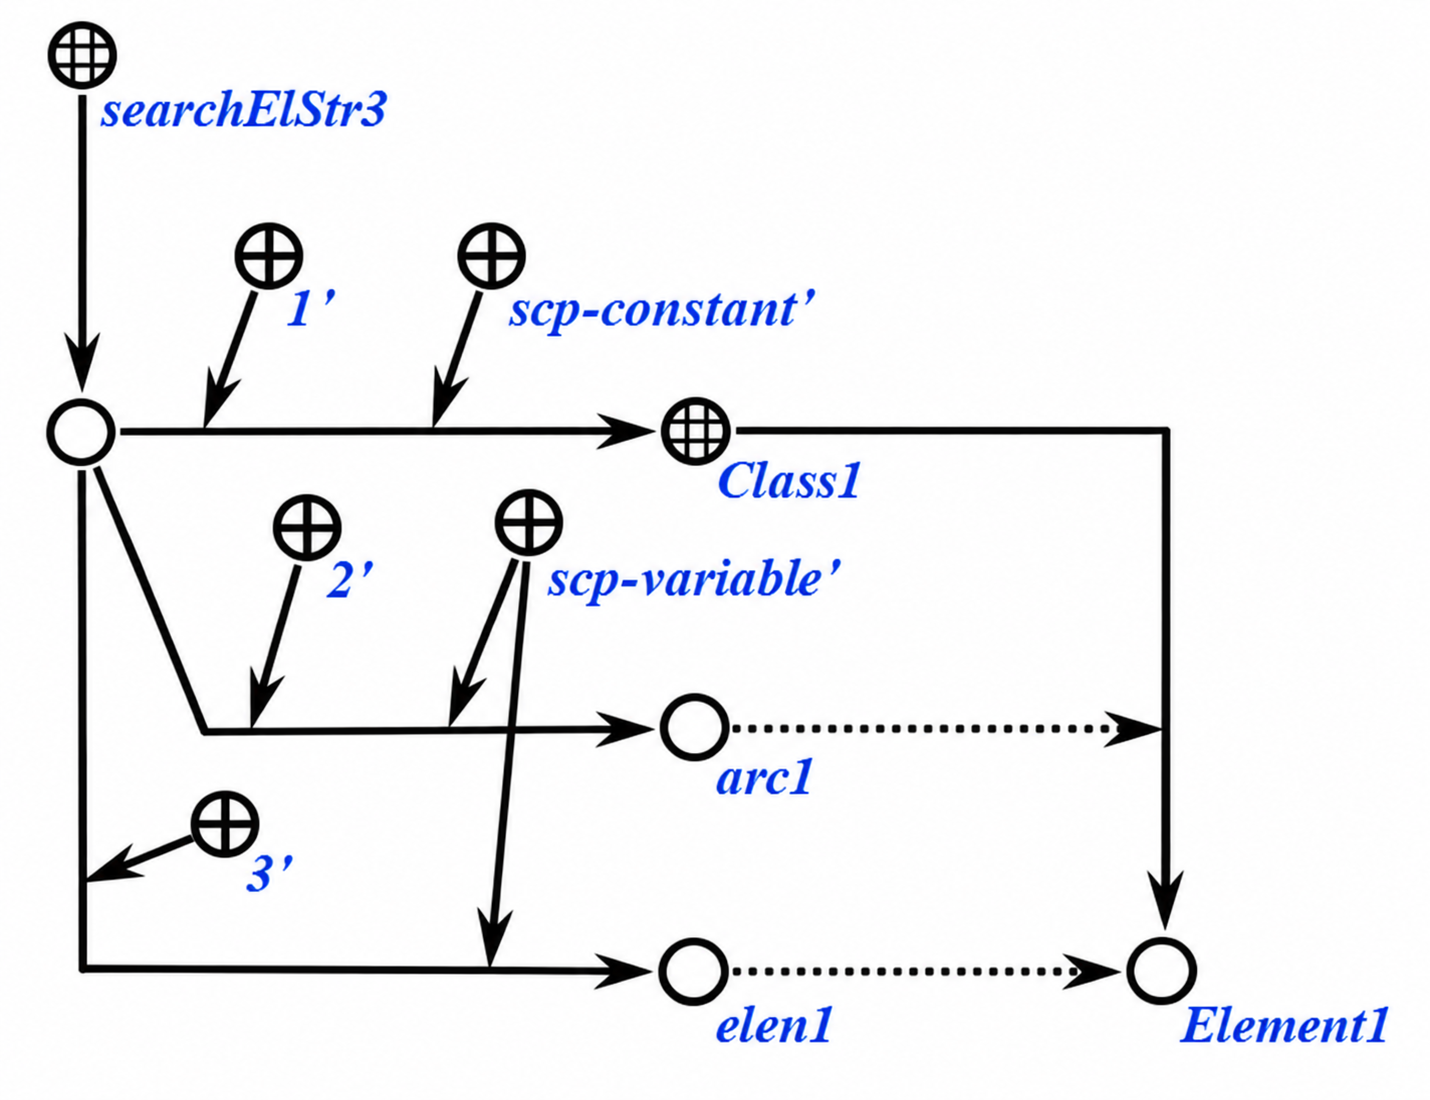
\includegraphics[width=189.00bp,height=145.42bp,keepaspectratio]{figures/sd_scp/scp_var_en.png}
	\end{center}

\end{frame}

\begin{frame}{\\Distinguish between}%
	\topline
	\RaggedRight

	\begin{SCn}
		\scnheader{sc-variable}
		\scntext{explanation}{Denotes an arbitrary sc-element from a specified set (the set of values). Used in logical formulas and generalized structures}

		\scnheader{scp-variable}
		\scntext{explanation}{Is a situational set that, at any time, either has no elements (the scp-variable has no value) or has exactly one element (the value of the scp-variable). Its value may be either an sc-variable or an sc-constant.}
	\end{SCn}

\end{frame}

\begin{frame}{\\sc-operand with an assigned value}
	\topline
	\RaggedRight
	\small
	\vspace{5mm}

	\begin{SCn}
	\scnheader{scp-operand with an assigned value\scnrolesign}
	\scntext{explanation}{The value of operands marked by the role relation \textit{scp-operand with an assigned value\scnrolesign} is considered assigned within the current \textit{scp-operator}. This value is taken into account during execution of the \textit{scp-operator} and remains unchanged after execution of the \textit{scp-operator}. Each \textit{scp-constant\scnrolesign} is considered by default an \textit{scp-operand with an assigned value\scnrolesign}, so explicitly using this role relation is redundant in that case. The operand itself is treated as its value. If the relation \textit{\mbox{scp-operand} with an assigned value\scnrolesign} marks an \textit{scp-variable\scnrolesign}, an attempt is made to find the value of that \textit{scp-variable\scnrolesign} (its element). If the attempt fails, a runtime error occurs and must be handled appropriately.

Any \textit{scp-operand with an assigned value\scnrolesign} regardless of the specific type of \textit{scp-operator} can be an \textit{scp-variable\scnrolesign}.}
	\end{SCn}

\end{frame}

\begin{frame}{\\scp-operand with an unassigned value}
	\topline
	\RaggedRight
	\small

	\begin{SCn}
		\scnheader{scp-operand with an unassigned value\scnrolesign}
		\scntext{explanation}{The value of operands marked by the role relation \textit{scp-operand with an unassigned value\scnrolesign} is considered unassigned within the current \textit{scp-operator}. At the start of execution of the \textit{scp-operator}, the connection between the \textit{scp-variable\scnrolesign} marked by this role relation and its element (value) is always deleted. Execution of this operator may either generate a new value for the \textit{scp-variable\scnrolesign} or leave it unassigned, in which case the \textit{scp-variable\scnrolesign} is considered to have no value. No \textit{scp-constant\scnrolesign} can be marked as an \textit{scp-operand with an unassigned value\scnrolesign} because a constant cannot change its value during interpretation of an \textit{scp-program}.}
	\end{SCn}

\end{frame}


\begin{frame}{\\Type of sc-element}
	\topline
	\RaggedRight
	\small
	\vspace{5mm}
	\begin{SCn}
		\scnheader{scp-operand\scnrolesign}
		\scnsuperset{type of sc-element\scnrolesign}
		\begin{scnindent}
			\begin{scnrelfromset}{partition}
				\scnitem{sc-node\scnrolesign}
				\begin{scnindent}
					\begin{scnrelfromset}{partition}
						\scnitem{structure\scnrolesign}
						\scnitem{relation\scnrolesign}
						\begin{scnindent}
						\scnsuperset{role relation\scnrolesign}
						\end{scnindent}
						\scnitem{class}
					\end{scnrelfromset}
				\end{scnindent}
				\scnitem{sc-arc\scnrolesign}
				\scnitem{sc-edge\scnrolesign}
				\scnitem{file\scnrolesign}
			\end{scnrelfromset}
			\begin{scnrelfromset}{partition}
				\scnitem{sc-constant\scnrolesign}
				\scnitem{sc-variable\scnrolesign}
			\end{scnrelfromset}
		\end{scnindent}
	\end{SCn}

\end{frame}

\begin{frame}{\\sc-arc}
	\topline
	\RaggedRight
	\begin{SCn}

		\scnheader{sc-arc\scnrolesign}
		\begin{scnrelfromset}{partition}
			\scnitem{general sc-arc\scnrolesign}
			\scnitem{sc-membership arc\scnrolesign}
			\begin{scnindent}
				\scnsuperset{basic sc-arc\scnrolesign}
			\end{scnindent}
			\begin{scnindent}
			\begin{scnrelfromset}{partition}
				\scnitem{positive sc-membership arc\scnrolesign}
				\scnitem{negative sc-membership arc\scnrolesign}
				\scnitem{fuzzy sc-membership arc\scnrolesign}
			\end{scnrelfromset}
			\begin{scnrelfromset}{partition}
				\scnitem{temporary sc-membership arc\scnrolesign}
				\scnitem{permanent sc-membership arc\scnrolesign}
			\end{scnrelfromset}
			\end{scnindent}
		\end{scnrelfromset}

	\end{SCn}
	\vspace{-3em}
\end{frame}

\begin{frame}{\\Example of an scp-search operator description}
	\topline
	\RaggedRight

	\begin{center}
		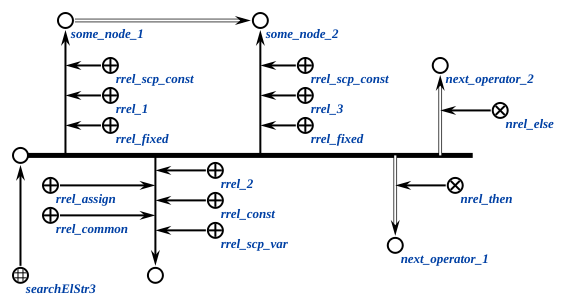
\includegraphics[scale=0.7]{figures/sd_scp/searchElStr3_faf.png}
	\end{center}

\end{frame}

\begin{frame}{\\Example of an scp-search operator description}
	\topline
	\RaggedRight

	\begin{center}
		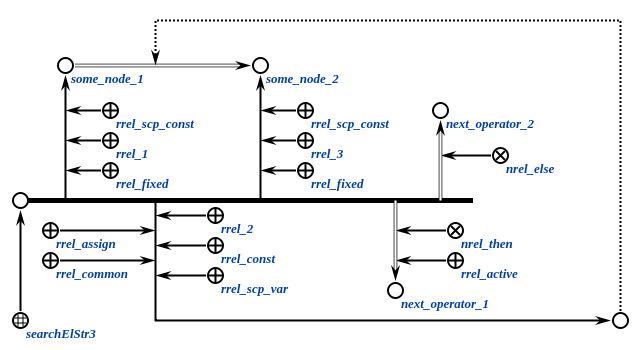
\includegraphics[scale=0.6]{figures/sd_scp/searchElStr3_faf_2.png}
	\end{center}

\end{frame}

\begin{frame}{\\Example of an scp-generation operator description}
	\topline
	\RaggedRight

	\vspace{10mm}

	\begin{center}
		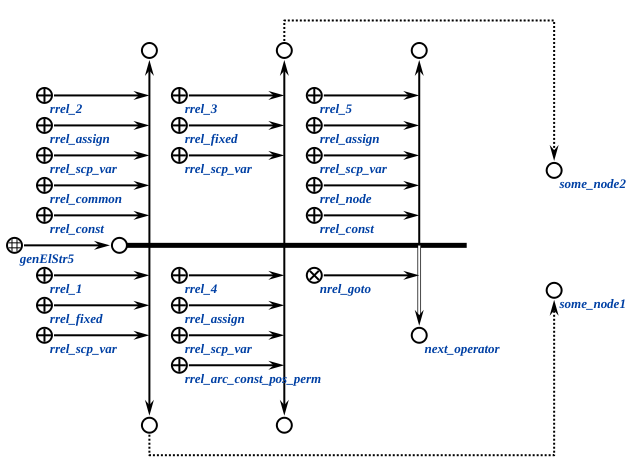
\includegraphics[scale=0.5]{figures/sd_scp/genElStr5_fafaa.png}
	\end{center}

\end{frame}

\begin{frame}{\\Example of an scp-generation operator description}
	\topline
	\RaggedRight

	\vspace{10mm}

	\begin{center}
		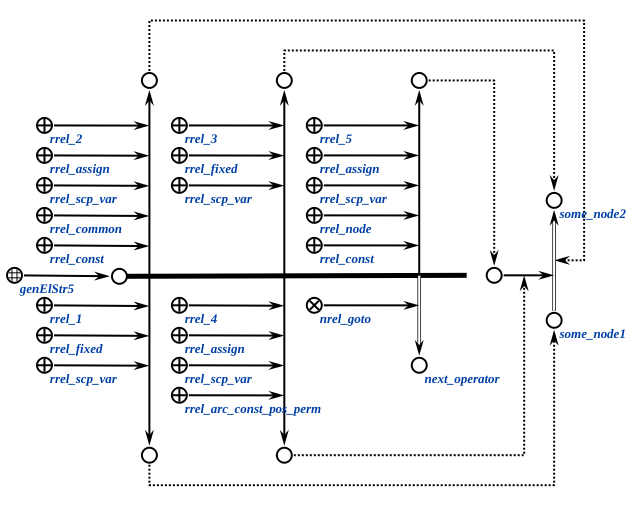
\includegraphics[scale=0.5]{figures/sd_scp/genElStr5_fafaa_2.png}
	\end{center}

\end{frame}

\begin{frame}{\\Transitions between scp-operators}
	\topline
	\RaggedRight

	\begin{textitemize}
		\item \textbf{\textit{goto*}}
		\item \textbf{\textit{then*}}
		\item \textbf{\textit{else*}}
	\end{textitemize}

\end{frame}

\begin{frame}{\\Transitions between scp-operators}
	\topline
	\RaggedRight

	\vspace{10mm}

	\begin{center}
	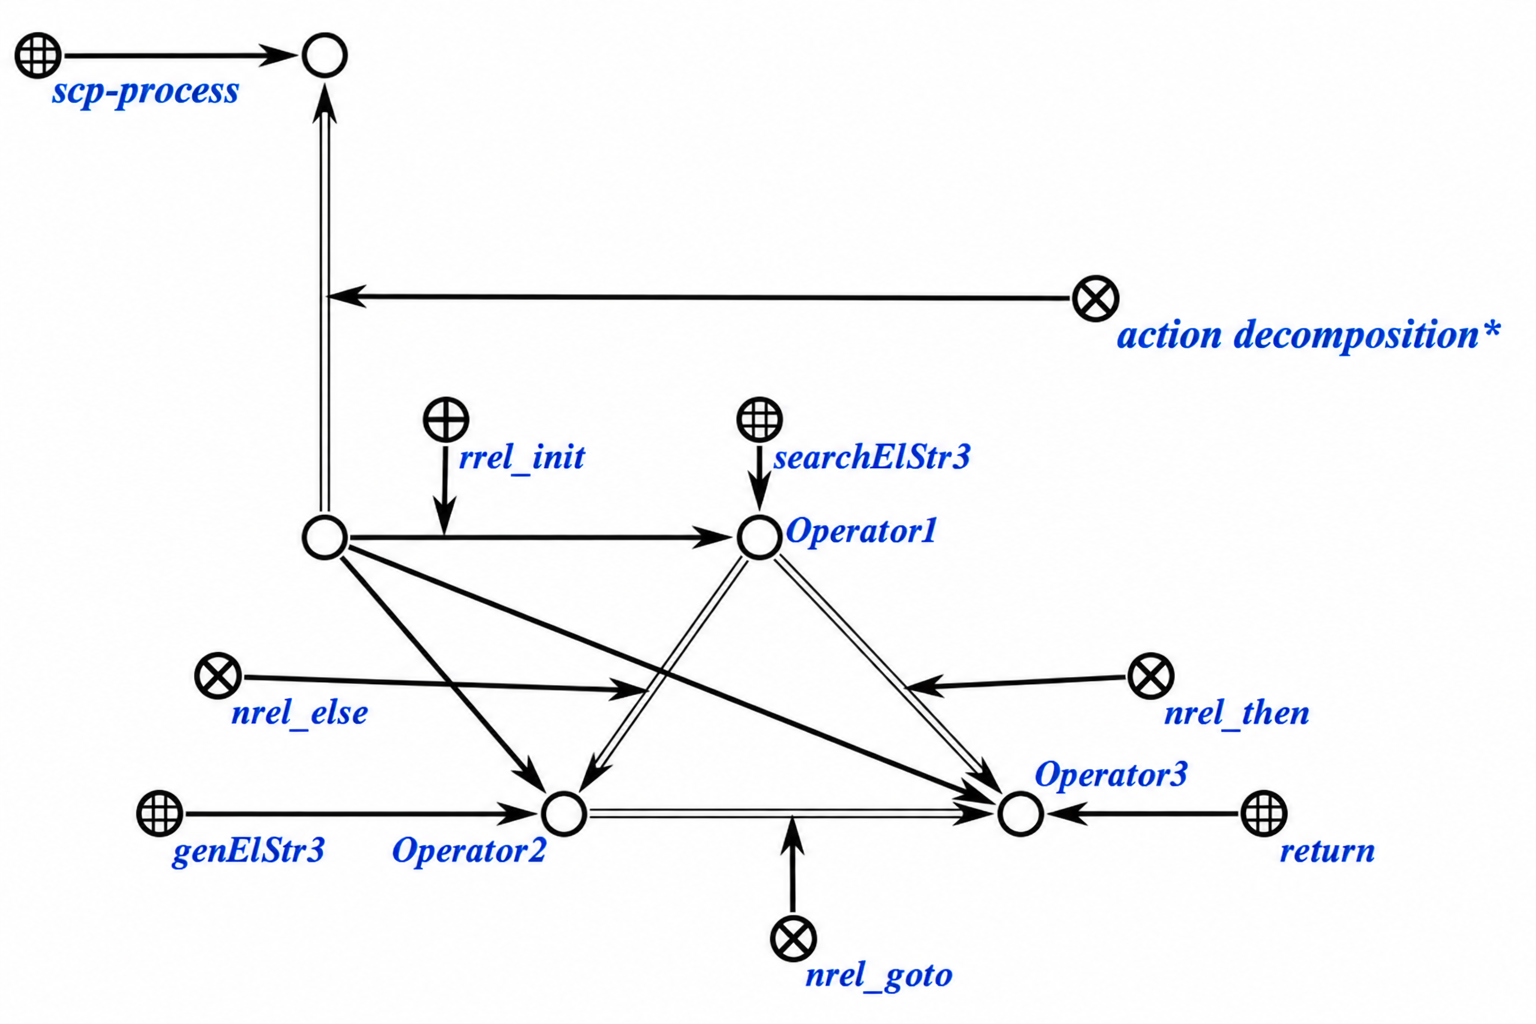
\includegraphics[width=297.67bp,height=198.45bp,keepaspectratio]{figures/sd_scp/operators_order1_en.png}
	\end{center}

\end{frame}

\begin{frame}{\\Transitions between scp-operators}
	\topline
	\RaggedRight

	\vspace{10mm}

	\begin{center}
		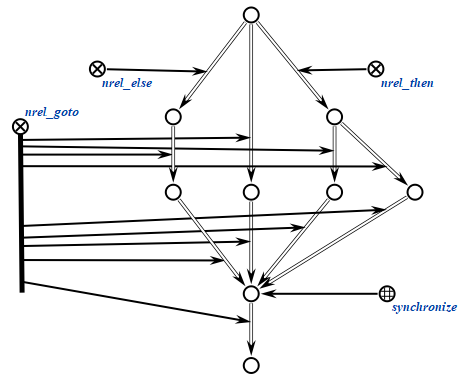
\includegraphics[scale=0.7]{figures/sd_scp/operators_order2.png}
	\end{center}

\end{frame}

\begin{frame}{\\Arguments of scp-processes and scp-programs}
	\topline
	\RaggedRight

	\begin{SCn}
		\scnheader{parameter of an scp-program\scnrolesign}
		\scnsubset{action argument\scnrolesign}
		\begin{scnrelfromset}{partition}
			\scnitem{in-parameter\scnrolesign}
			\scnitem{out-parameter\scnrolesign}
		\end{scnrelfromset}
	\end{SCn}

	The role relation \textbf{\textit{parameter of an scp-program\scnrolesign}} connects the sign of the \textit{\mbox{scp-process}} corresponding to an \textit{scp-program} to its arguments.

\end{frame}


\begin{frame}{\\\textit{in-parameter\scnrolesign}}
	\topline
	\RaggedRight

	Parameters of type \textbf{\textit{in-parameter\scnrolesign}}, although they correspond to \textit{scp-program variables\scnrolesign}, cannot change their value during interpretation. A fixed value is assigned when a unique copy of the \textit{scp-program} (\textit{scp-process}) is created for interpretation; thus the corresponding \textit{scp-variable\scnrolesign} becomes an \textit{scp-constant\scnrolesign} within each \textit{scp-operator} in which that \textit{scp-variable\scnrolesign} occurs, before interpretation begins. The use of \textit{in-parameters} is analogous to a variant of pass-by-value in conventional programming languages, with the condition that the local variable's value in the child program cannot be changed.

\end{frame}

\begin{frame}{\\\textit{out-parameter\scnrolesign}}
	\topline
	\RaggedRight

	\vspace{10mm}

	Parameters of type \textbf{\textit{out-parameter\scnrolesign}} correspond to \textit{scp-program variables\scnrolesign} and have the same properties. Usually, the value of this parameter is needed by the parent \textit{scp-program} containing the operator that calls the current \textit{scp-program}. At the start of interpretation, the node denoting the parent process's variable (more precisely, its unique copy within the process) is passed to the child process. That variable may or may not already have a value. During and after the child process's interpretation, the parent process can continue to work with the variable passed as an \textit{out-parameter\scnrolesign}, viewing or modifying its value as needed. An out-parameter is analogous to pass-by-reference in conventional \textit{programming languages}.

\end{frame}

\begin{frame}{\\Action of interpreting an scp-program}
	\topline
	\RaggedRight

	\begin{center}
		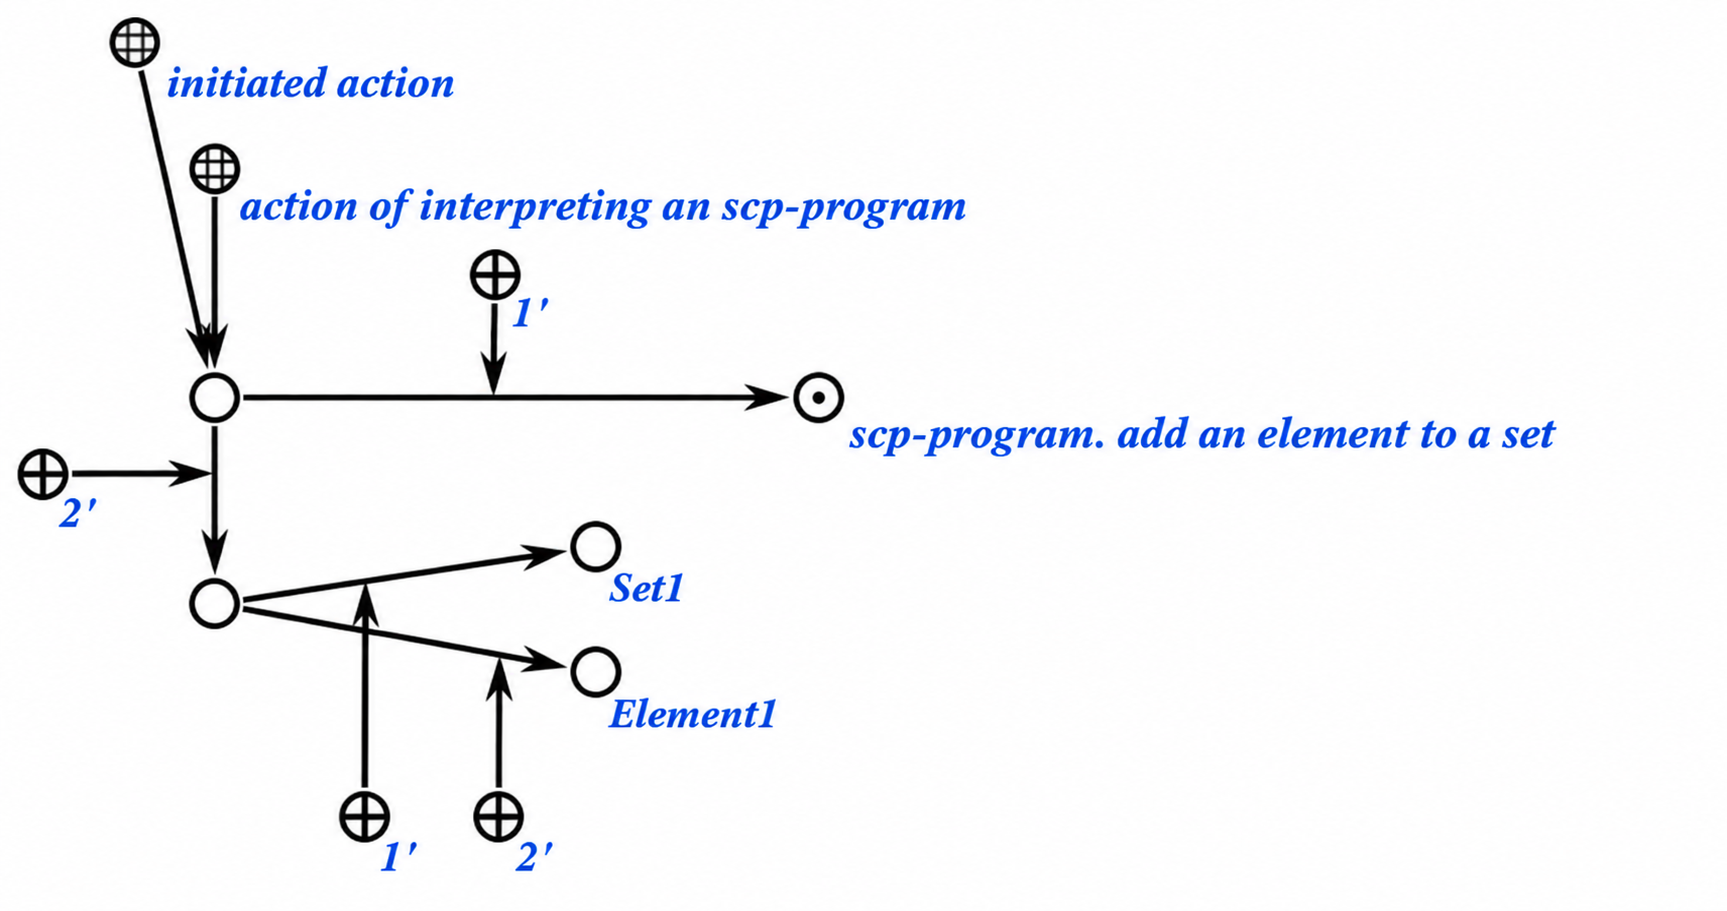
\includegraphics[width=304.50bp,height=160.65bp,keepaspectratio]{figures/sd_scp/interpreting_action_en.png}
	\end{center}

\end{frame}

\begin{frame}{\\Principles of scp-program interpretation}
	\topline
	\RaggedRight

	\vspace{10mm}

	\begin{textitemize}
		\item A specific scp-process is generated using the scp-program as a template
		\begin{textitemize}
			\item The sc-variables corresponding to \textit{in-parameters\scnrolesign} are replaced with the specific arguments of the \textit{action of interpreting the scp-program}
			\item The sc-variables corresponding to \textit{out-parameters\scnrolesign} are replaced with scp-operands that are arguments of the \textit{action of interpreting the scp-program}
			\item For the corresponding \textit{in-parameters\scnrolesign} the scp-operand role changes from \textit{scp-variable\scnrolesign} to \textit{scp-constant\scnrolesign}
		\end{textitemize}
		\item ...
	\end{textitemize}

\end{frame}

\begin{frame}{\\Principles of scp-program interpretation}
	\topline
	\RaggedRight

	\vspace{10mm}

	\begin{textitemize}
		\item ...
		\item The initial scp-operator of the resulting scp-process is located and initiated (added to the set of \textit{active scp-operators})
		\item After an scp-operator is executed, the next scp-operators are located and initiated, depending on whether execution succeeded
		\item This continues until the scp-operator for program termination (return) is encountered
	\end{textitemize}

\end{frame}

\begin{frame}{Implementing loops\\Problems}
	\topline
	\RaggedRight

	\begin{textitemize}
		\item Sets in SC-code are unordered by default.
		\item sc-memory has no built-in mechanism for iterating over set elements, since this requires additional auxiliary constructions. This follows from the nonlinearity of sc-memory.
		\item \textit{scp-operator for associative construction search} finds \underline{one} arbitrary construction matching a given pattern.
		\item To find another (the ``next'') construction matching the same pattern, the previous one would have to be destroyed so that it is no longer found. This, however, would damage the sc-construction being processed.
	\end{textitemize}

\end{frame}

\begin{frame}{Implementing loops\\Proposed approach}
	\topline
	\RaggedRight

	\begin{textitemize}
		\item Find all sc-constructions matching a given pattern and place the required components in a temporary set
		\item Take elements from the temporary set one at a time, process them, and remove each processed element from the set
		\item Finally, delete the temporary set itself
	\end{textitemize}

\end{frame}

\begin{frame}{generated set\scnrolesign}
	\topline
	\RaggedRight

	\begin{SCn}

		\scnheader{scp-operand\scnrolesign}
		\scnsuperset{generated set\scnrolesign}

			\begin{scnindent}
				\begin{scnrelfromset}{partition}
					\scnitem{generated set 1\scnrolesign}
					\scnitem{generated set 2\scnrolesign}
					\scnitem{generated set 3\scnrolesign}
					\scnitem{generated set 4\scnrolesign}
					\scnitem{generated set 5\scnrolesign}
				\end{scnrelfromset}
			\end{scnindent}

	\end{SCn}
\end{frame}


\begin{frame}{scp-operator for three-element construction search with set formation}
	\topline
	\RaggedRight
	\vspace{10mm}

	\begin{center}
		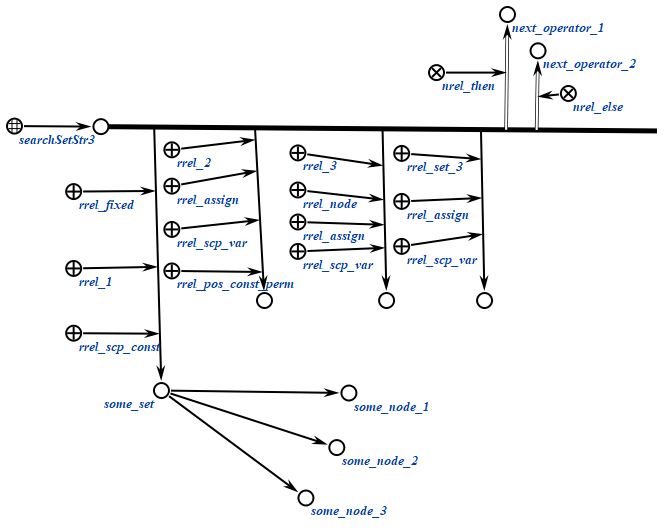
\includegraphics[scale=0.55]{figures/sd_scp/searchSetStr3.png}
	\end{center}

\end{frame}

\begin{frame}{scp-operator for three-element construction search with set formation}
	\topline
	\RaggedRight
	\vspace{10mm}

	\begin{center}
		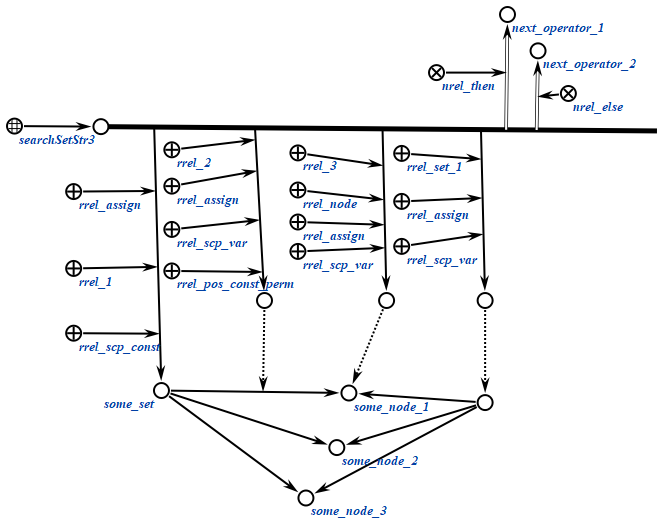
\includegraphics[scale=0.55]{figures/sd_scp/searchSetStr3_2.png}
	\end{center}

\end{frame}

\begin{frame}{scp-operator for three-element construction search with set formation}
	\topline
	\RaggedRight
	\vspace{10mm}

	\begin{center}
		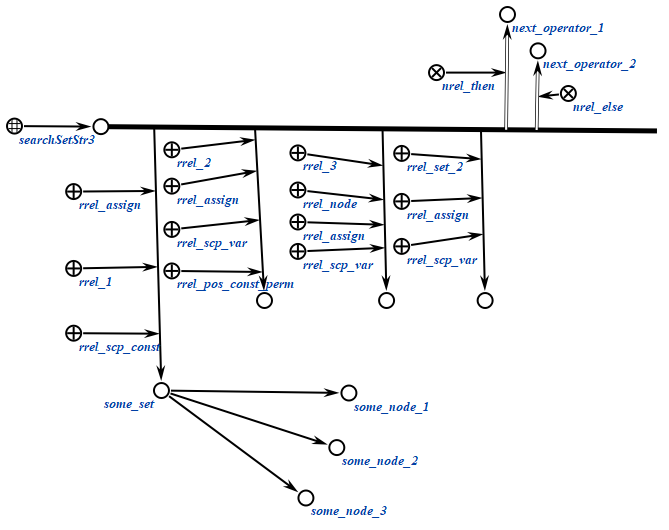
\includegraphics[scale=0.55]{figures/sd_scp/searchSetStr3_3.png}
	\end{center}

\end{frame}

\begin{frame}{scp-operator for three-element construction search with set formation}
	\topline
	\RaggedRight
	\vspace{10mm}

	\begin{center}
		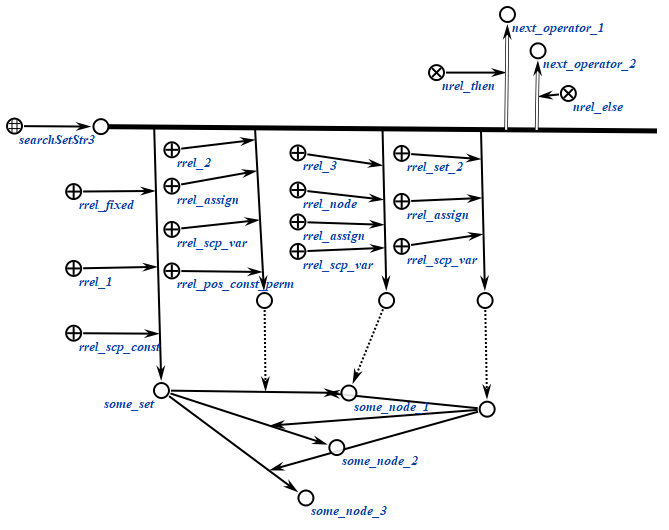
\includegraphics[scale=0.55]{figures/sd_scp/searchSetStr3_4.png}
	\end{center}

\end{frame}

\begin{frame}{scp-operator for three-element construction search with set formation}
	\topline
	\RaggedRight
	\vspace{10mm}

	\begin{center}
		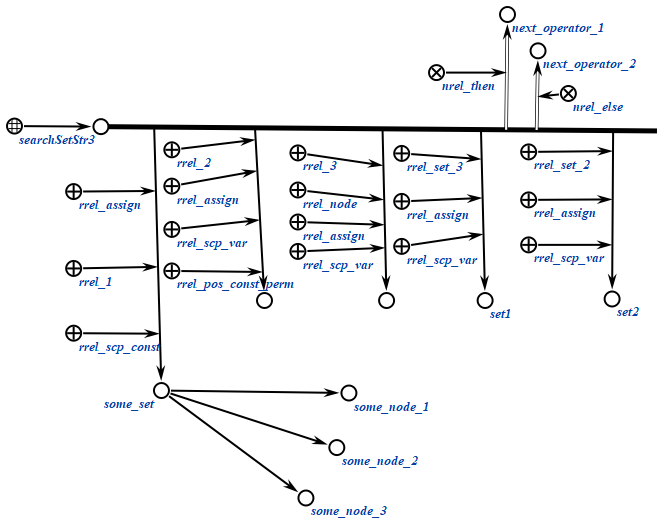
\includegraphics[scale=0.55]{figures/sd_scp/searchSetStr3_5.png}
	\end{center}

\end{frame}

\begin{frame}{scp-operator for three-element construction search with set formation}
	\topline
	\RaggedRight
	\vspace{10mm}

	\begin{center}
		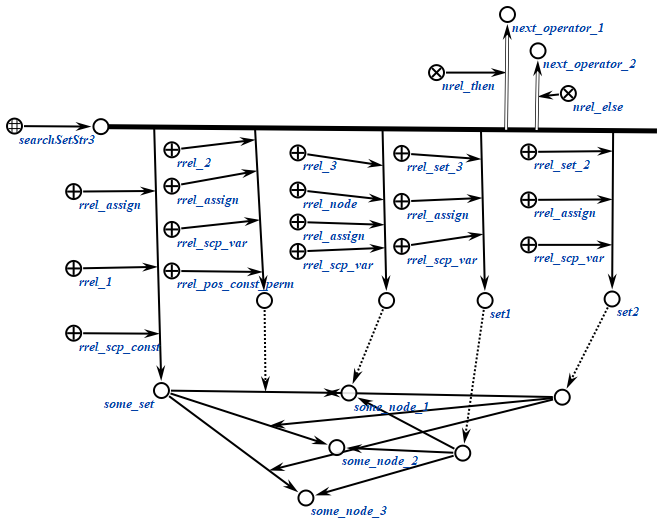
\includegraphics[scale=0.55]{figures/sd_scp/searchSetStr3_6.png}
	\end{center}

\end{frame}

\begin{frame}{scp-operator for three-element construction search with set formation}
	\topline
	\RaggedRight
	\vspace{10mm}

	\begin{center}
		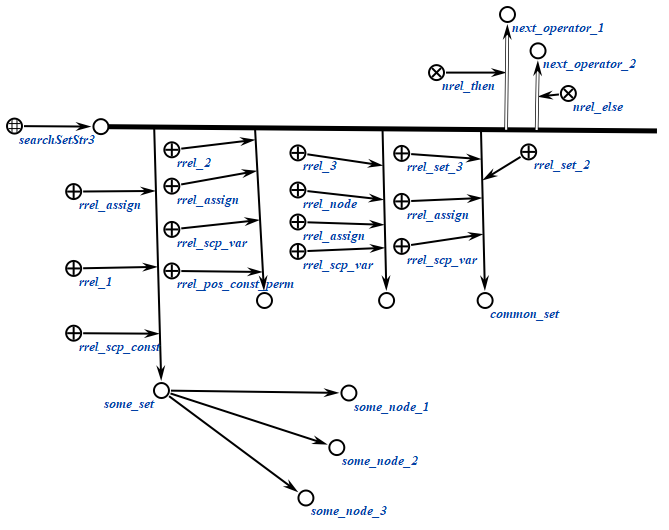
\includegraphics[scale=0.55]{figures/sd_scp/searchSetStr3_7.png}
	\end{center}

\end{frame}

\begin{frame}{scp-operator for three-element construction search with set formation}
	\topline
	\RaggedRight
	\vspace{10mm}

	\begin{center}
		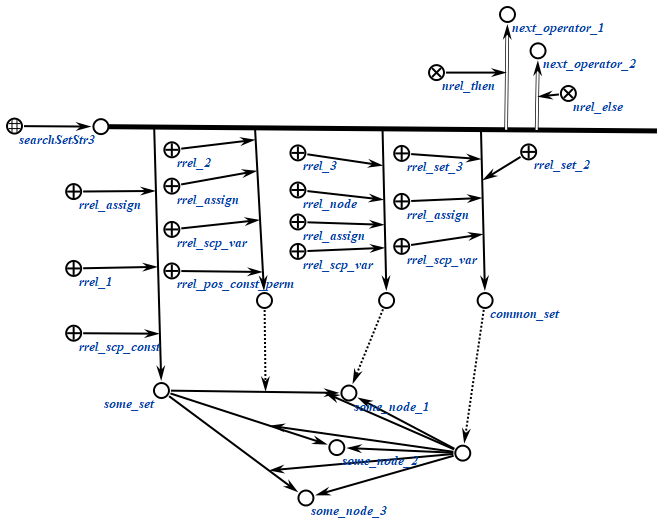
\includegraphics[scale=0.55]{figures/sd_scp/searchSetStr3_8.png}
	\end{center}

\end{frame}

\begin{frame}{\\Example of loop execution}
	\topline
	\RaggedRight
	\vspace{10mm}

	\begin{center}
		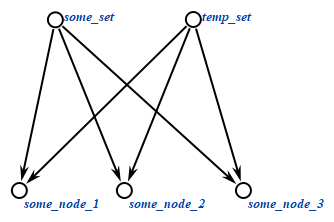
\includegraphics[scale=0.8]{figures/sd_scp/cycle1.png}
	\end{center}

\end{frame}

\begin{frame}{\\Example of loop execution}
	\topline
	\RaggedRight
	\vspace{10mm}

	\begin{center}
		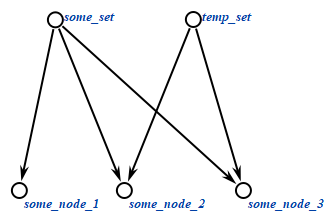
\includegraphics[scale=0.8]{figures/sd_scp/cycle2.png}
	\end{center}

\end{frame}

\begin{frame}{\\Example of loop execution}
	\topline
	\RaggedRight
	\vspace{10mm}

	\begin{center}
		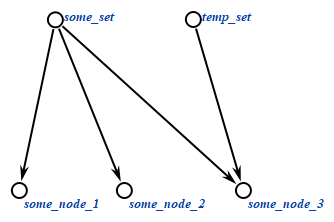
\includegraphics[scale=0.8]{figures/sd_scp/cycle3.png}
	\end{center}

\end{frame}

\begin{frame}{\\Example of loop execution}
	\topline
	\RaggedRight
	\vspace{10mm}

	\begin{center}
		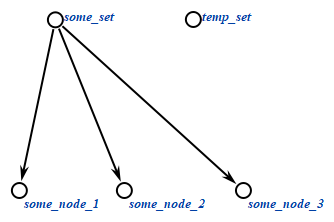
\includegraphics[scale=0.8]{figures/sd_scp/cycle4.png}
	\end{center}

\end{frame}

\begin{frame}{\\Loop structure}
	\topline
	\RaggedRight
	\vspace{10mm}

	\begin{center}
		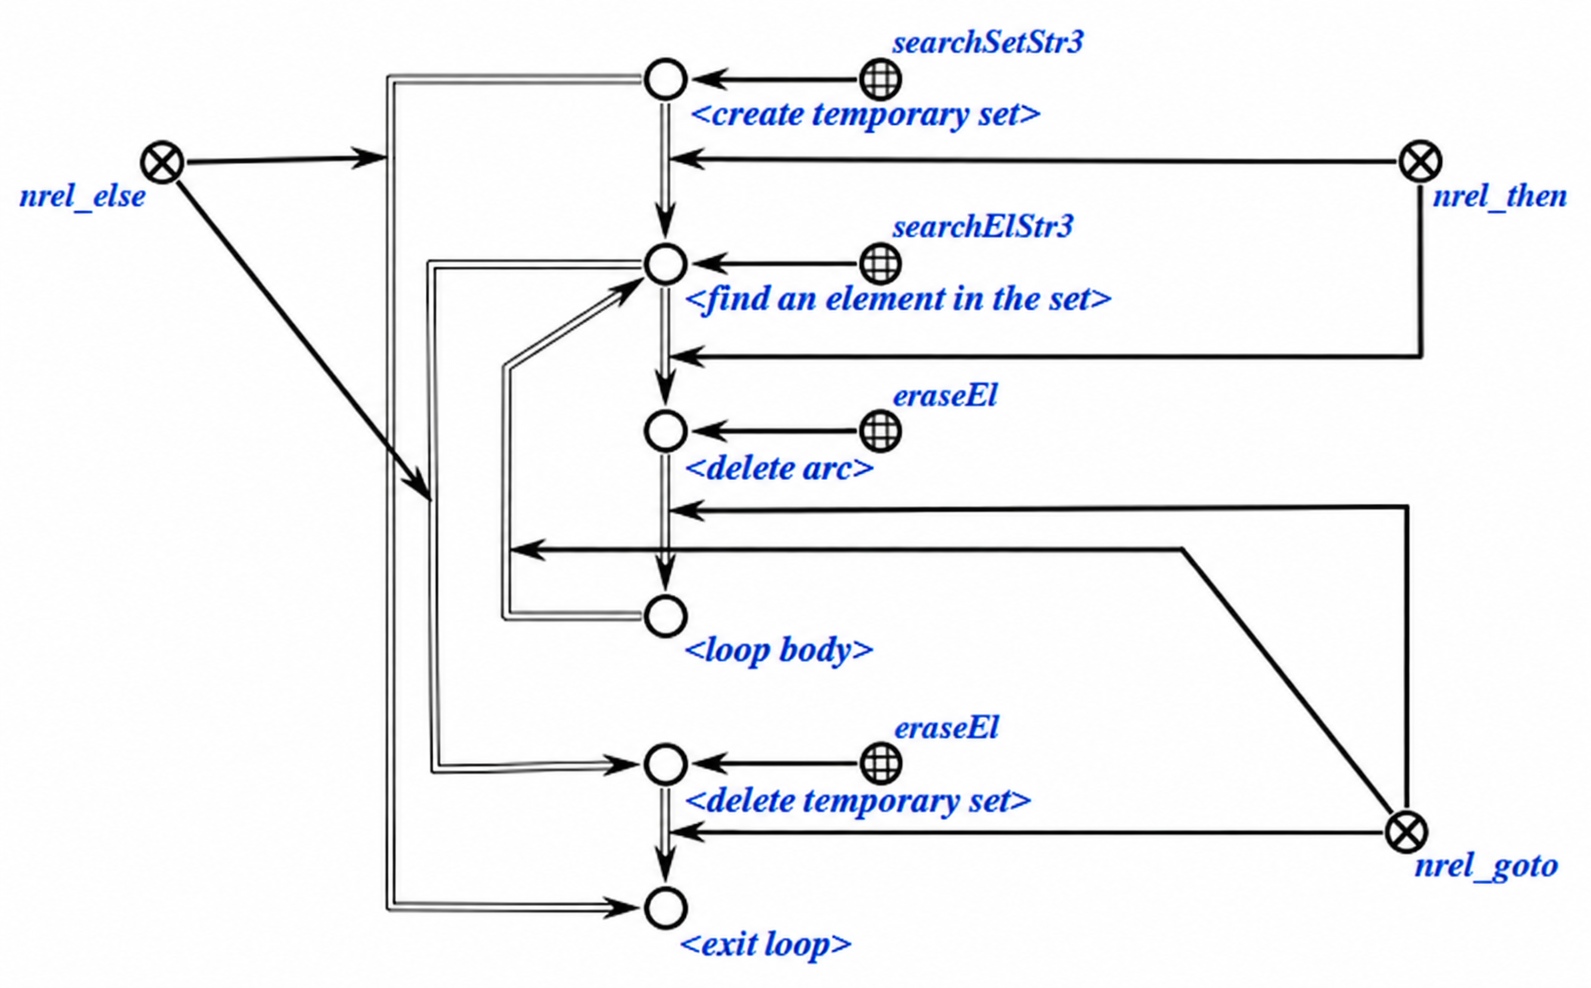
\includegraphics[width=331.27bp,height=205.80bp,keepaspectratio]{figures/sd_scp/cycle_operators_en.png}
	\end{center}

\end{frame}

\begin{frame}{\\Loop structure}
	\topline
	\RaggedRight
	\vspace{10mm}

	\begin{center}
		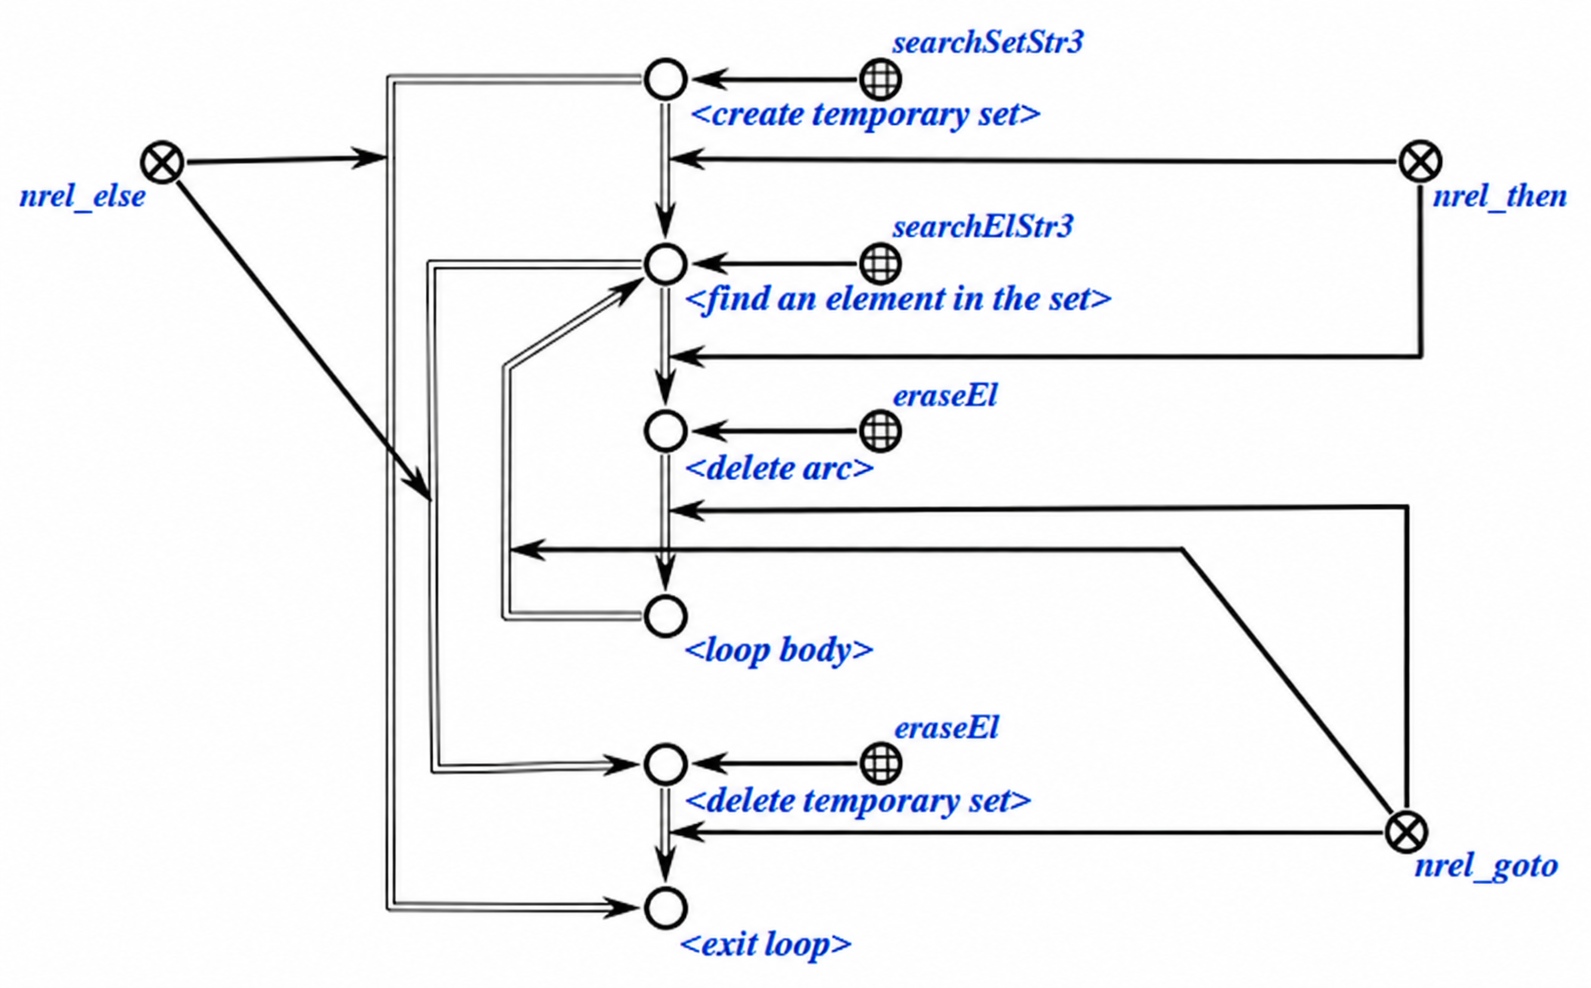
\includegraphics[width=331.27bp,height=205.80bp,keepaspectratio]{figures/sd_scp/cycle_operators_en.png}
	\end{center}

\end{frame}

\begin{frame}{\\Calling subroutines}
	\topline
	\RaggedRight
	\vspace{10mm}

	\begin{center}
		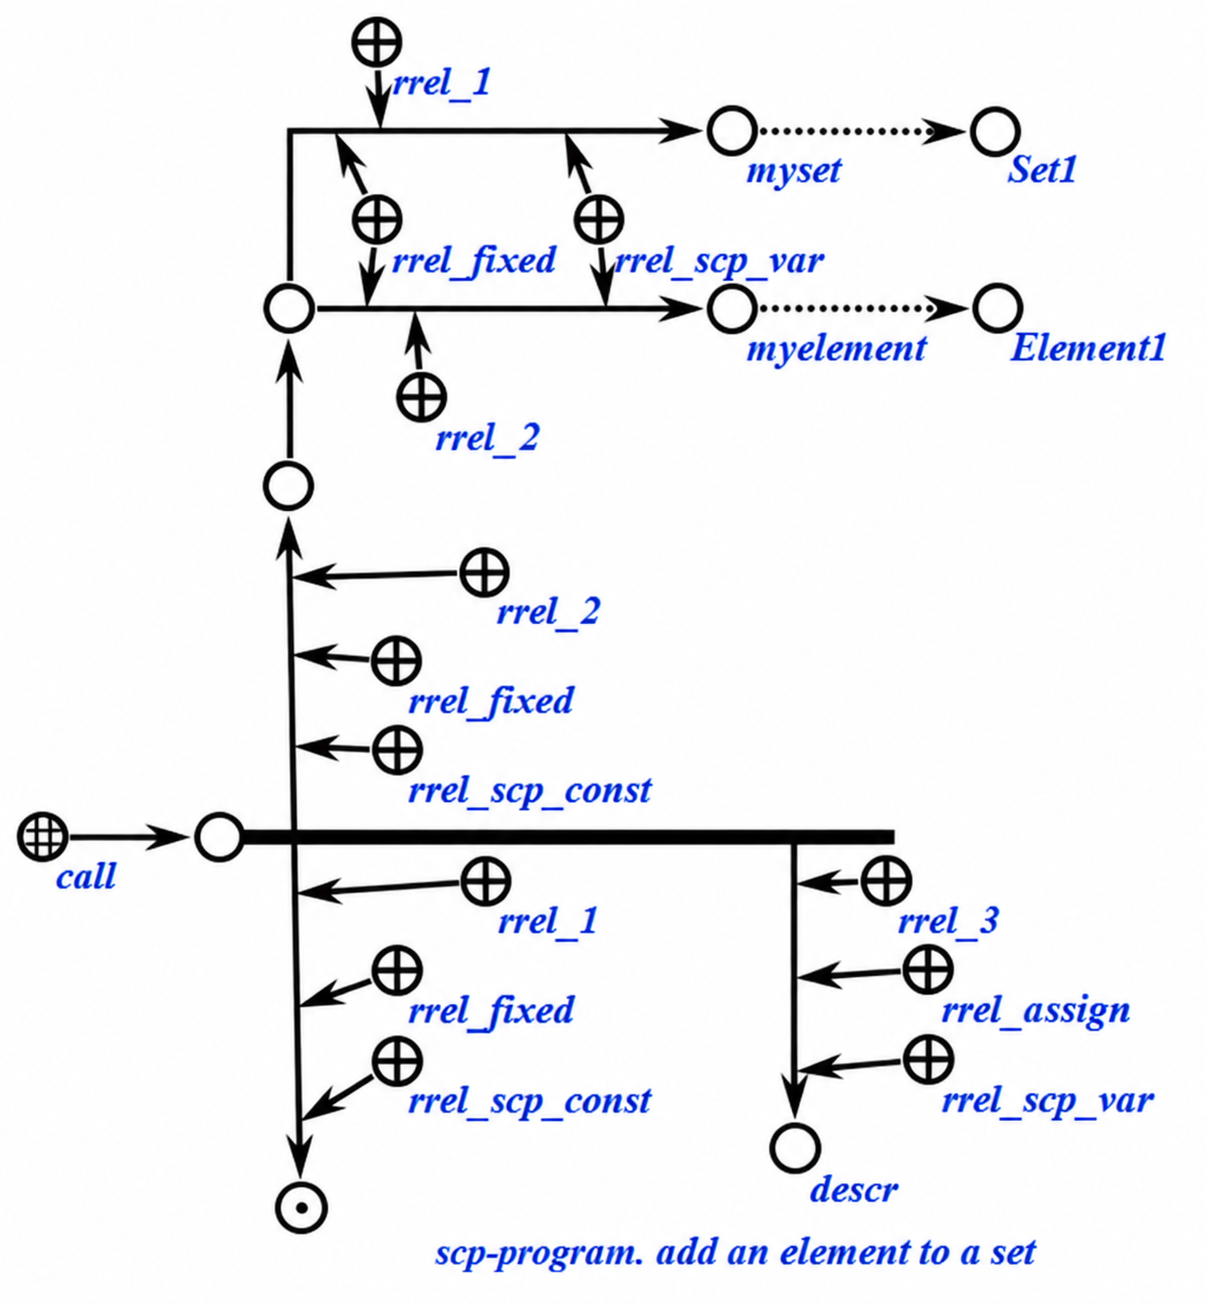
\includegraphics[width=167.89bp,height=181.50bp,keepaspectratio]{figures/sd_scp/call_en.png}
	\end{center}

\end{frame}

\begin{frame}{\\Calling subroutines}
	\topline
	\RaggedRight
	\vspace{10mm}


	\begin{center}
		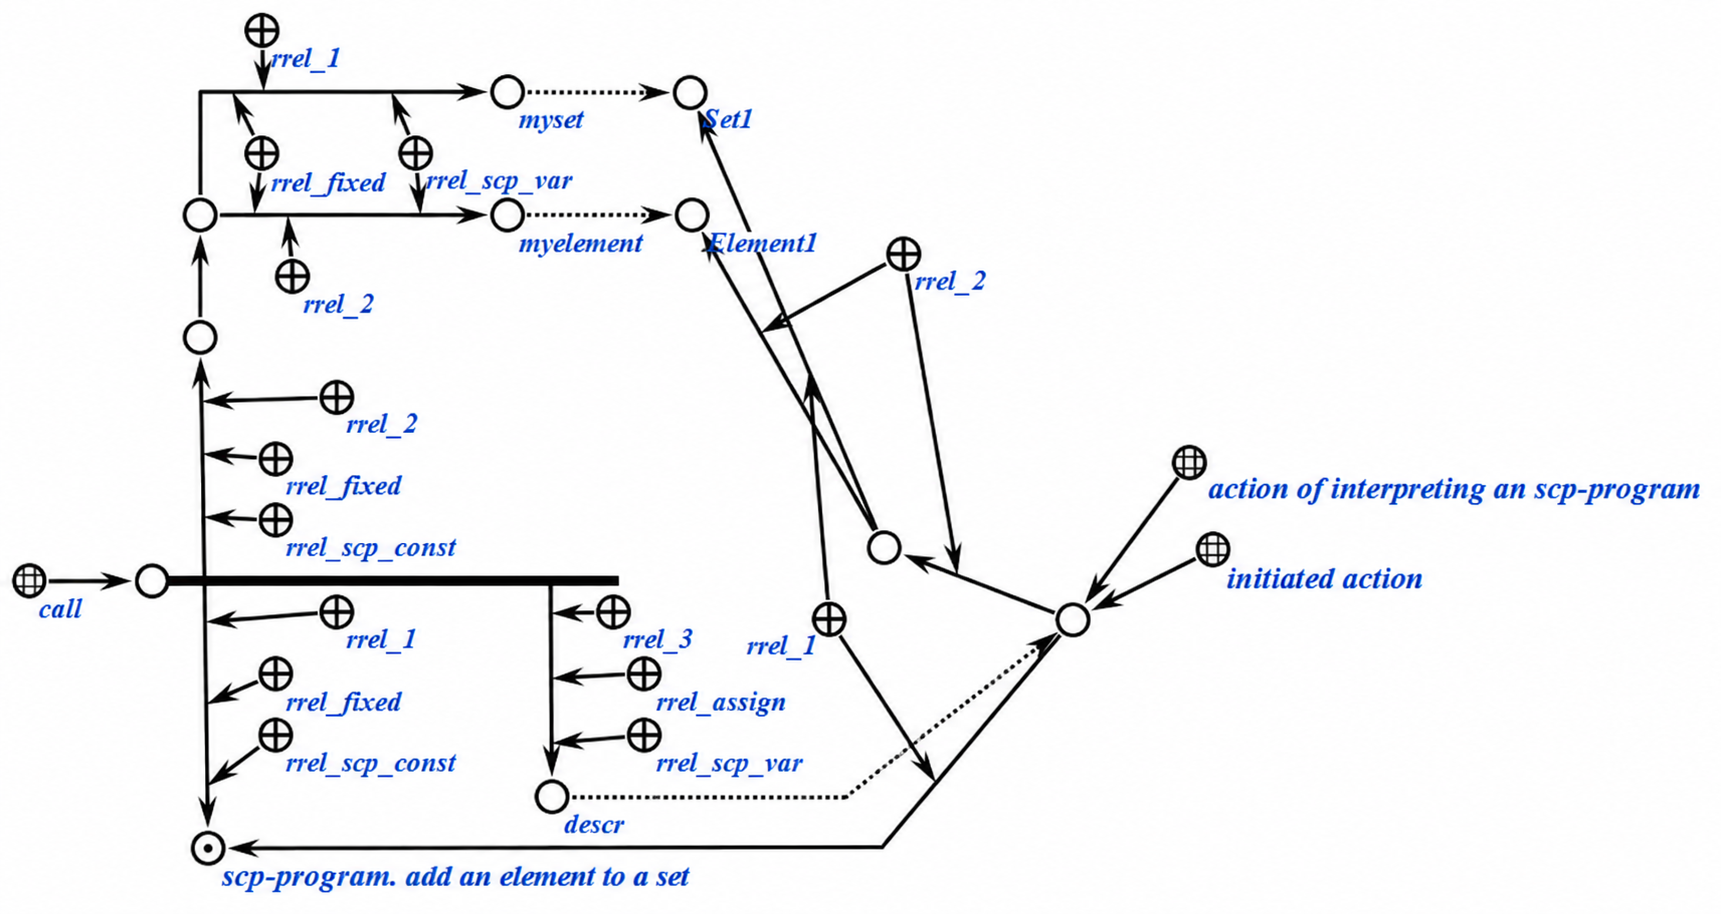
\includegraphics[width=319.75bp,height=169.60bp,keepaspectratio]{figures/sd_scp/call2_en.png}
	\end{center}

\end{frame}

\begin{frame}{\\Calling subroutines}
	\topline
	\RaggedRight
	\vspace{10mm}

	\begin{center}
		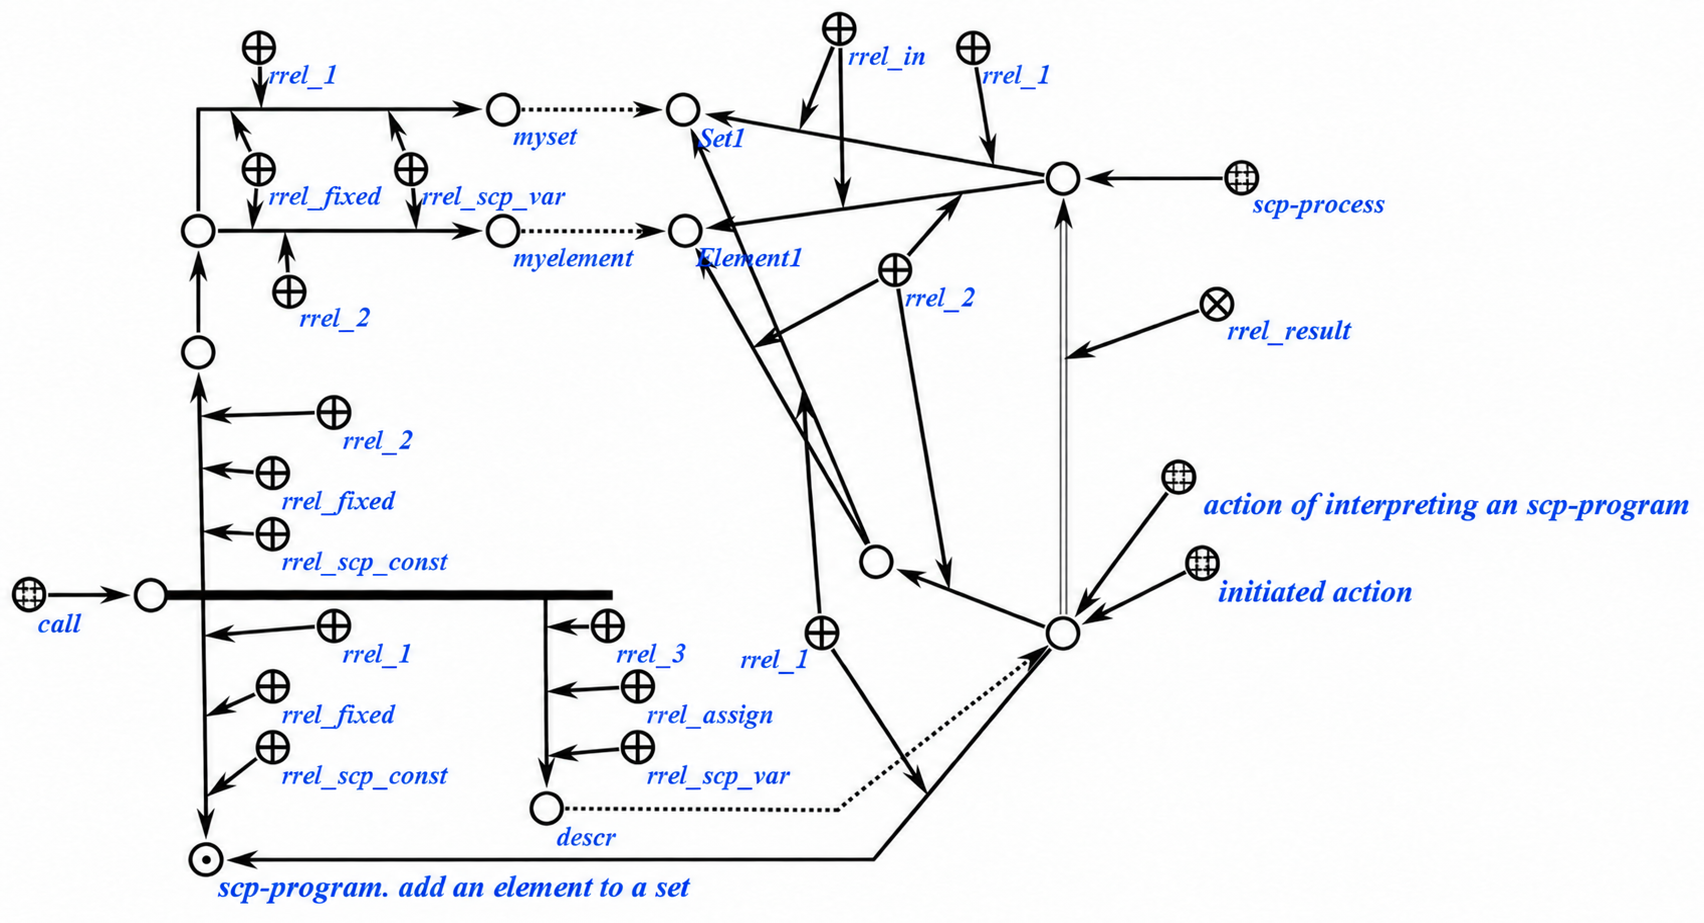
\includegraphics[width=319.75bp,height=173.41bp,keepaspectratio]{figures/sd_scp/call3_en.png}
	\end{center}

\end{frame}

\begin{frame}{\\Waiting for a subroutine to finish}
	\topline
	\RaggedRight
	\vspace{10mm}

	\begin{center}
		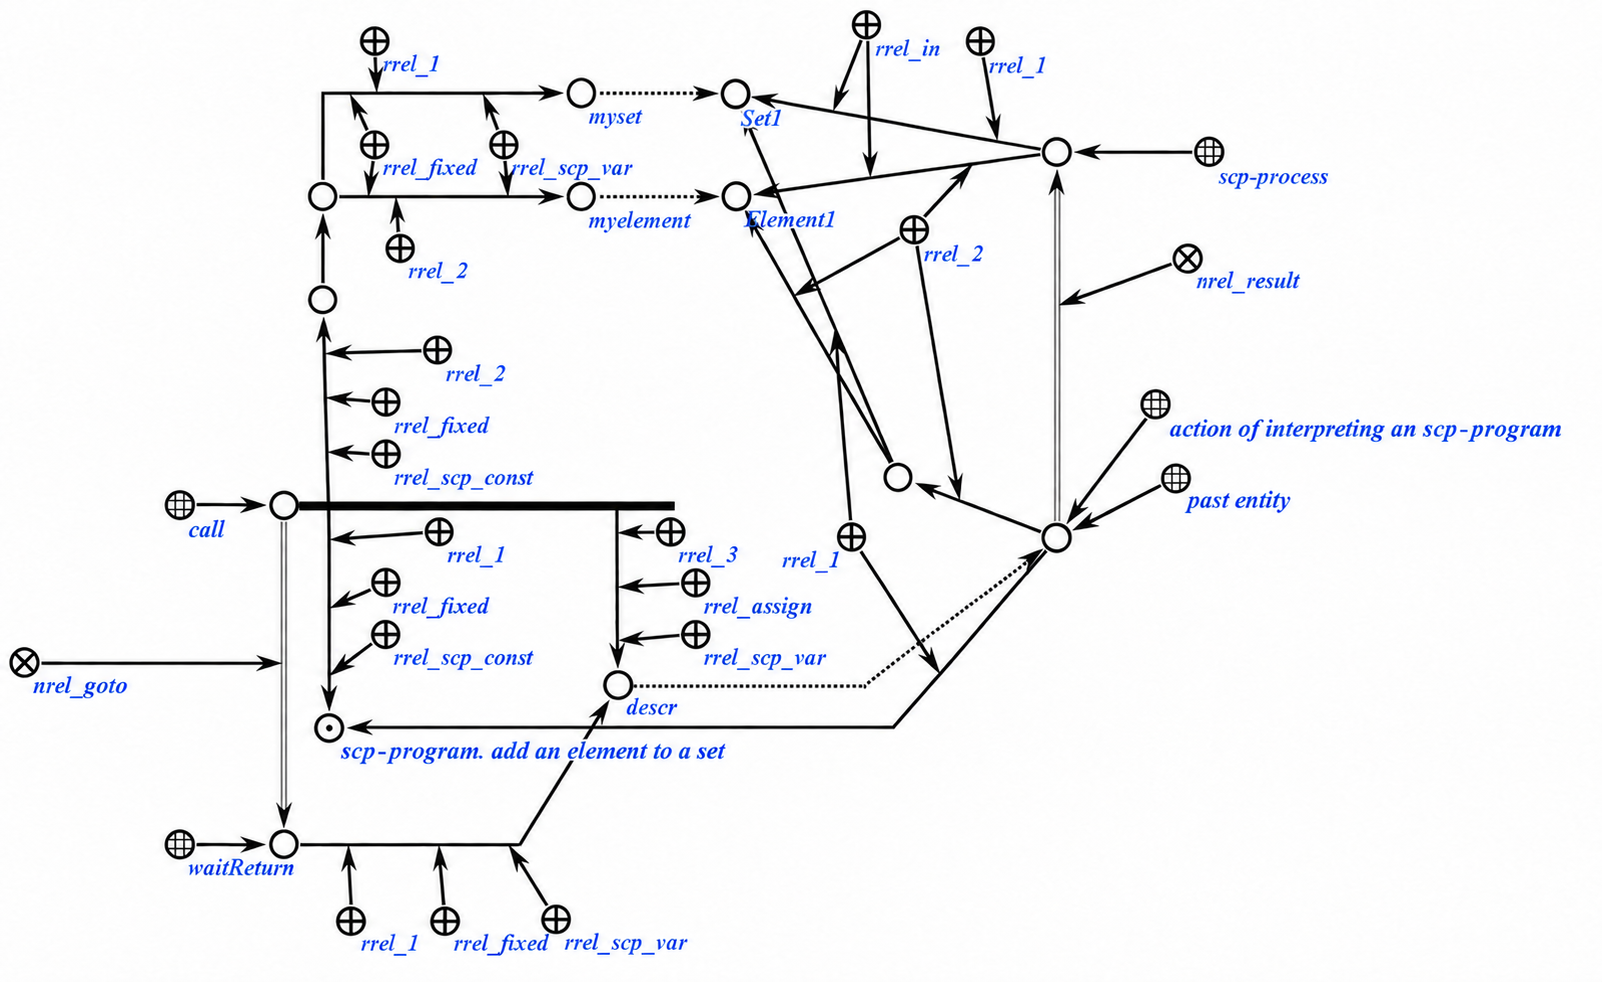
\includegraphics[width=306.45bp,height=187.70bp,keepaspectratio]{figures/sd_scp/waitReturn_en.png}
	\end{center}

\end{frame}

\begin{frame}{\\Agent scp-program}
	\topline
	\RaggedRight
	\scnheader{agent scp-program}
	\scnsubset{scp-program}
	\scntext{explanation}{\textit{scp-programs} of this class implement knowledge-processing agent programs and have a strictly fixed set of parameters. Each has exactly two \textit{in-parameters\scnrolesign}. The first parameter's value is the sign of a binary ordered pair that is the second component of a tuple of the \textit{primary initiation condition*} relation for the abstract \textit{sc-agent} whose set of \textit{sc-agent programs*} contains the \textbf{\textit{agent scp-program}} under consideration. It essentially describes the class of events to which that sc-agent responds.

The second parameter's value is an \textit{sc-element} directly associated with the event that initiated the corresponding \textit{sc-agent}, for example, a generated or deleted \textit{sc-arc} or \textit{sc-edge}.}
	\vspace{-2em}
\end{frame}
